\section{Empirical Analysis}

\subsection{Data}
\paragraph*{Auction Records.} For the auction bids, we obtained the data directly from Arbitrum's database \cite{offchainlabs2025howtousetimeboost}. Our sample spans bids from May to October 2025. While multiple bidders participate, we focus on the two most dominant participants, \texttt{0x8c6f} and \texttt{0x95c0}, who together win over $90\%$ of rounds between May and October. 

\paragraph*{Measuring Volatility.} We proxy market-wide volatility using high-frequency ETH price data from Binance. As ETH is the most liquid crypto-asset on Arbitrum\footnote{We exclude stablecoins; see \cite{l2beat}.}, focusing on ETH serves as a low-friction approximation of overall market conditions. While price follows a stochastic process and thus the integrated variance is also essentially random, all we have is historical data of a single \emph{realized} path out of all possible outcomes. Therefore, we have to estimate $\E[\IV]$ and $\Var(\IV)$ from the given path of price. We adopt a standard approach, treating the realized variance (RV), the sum of squares of log returns $r_t$, as $\widehat{\E[\IV]}$, while estimating $\widehat{\Var(\IV)}$ with the following Newey-West estimator: \[
\widehat{\Var(\IV)} = T (\gamma_0 + 2\sum_{k=1}^L w_k \gamma_k),
\] where \[
\gamma_k \equiv \frac{1}{T} \sum_{t=1}^{T - k} (r^2_{t + k} - \overline{r^2})(r^2_t - \overline{r^2}) \quad \text{and} \quad \overline{r^2} \equiv \frac{1}{T} \sum_{t=1}^T r_t^2\, ,
\] for $k = 0, 1, 2, \cdots$, and $w_k \equiv 1 - \frac{k}{L + 1}$ is weight function. The standard practice of setting \(L \) is of \( L = \mathcal O(T^{1/3})\). In our setting, we set $T = 60$ and $L = 5$.

\paragraph*{Bidder Forecasts.} The theoretical model proposed in \cref{sec:theory} posits that bids depend on bidders' private forecasts of realized variance, which are unobservable. We therefore adopt the following assumption to bridge the theory with our ex-post volatility measures:

\begin{assump}[On-average Correct Forecast]
    Bidders are capable of \emph{on-average} correctly forecasting the mean and variance of forthcoming $\IV_r$ based on public and private information available at time $D_r$. That is, for \[
         \epsilon_{ir} \equiv m^{\IV}_{ir} - \E[\IV_r] \quad and \quad \tau_{ir} \equiv v^{\IV}_{ir} - \Var(\IV_r),
    \] \( \E \left[ \epsilon_{ir} | \mathcal F_r \right] = \E \left[ \tau_{ir} | \mathcal F_r\right] = 0\).\footnote{Note that this does not necessarily violate the CIPV framework. One can interpret this assumption that, based on public information, it is possible to, on average, correctly forecast the mean and variance of $\IV$. Then $\epsilon_{ir}$ and $\tau_{ir}$ being independent and private is sufficient for the CIPV setting.} % TODO: replace RQ - RV^2 with Newey-West Estimator, and RV with RV/sqrt(P)
\end{assump}
\noindent This errors-in-variables framework implies that our estimates of $\theta_1$ and $\theta_2$ will be subject to attenuation bias, which will bias them towards zero. Consequently, finding statistically significant coefficients despite this bias would provide a conservative and even stronger confirmation of our hypotheses.

\subsection{Estimation}
Our dependent variable, the observed bid $b_{ir}$, is left-censored at the reserve price $C = 0.001$ ETH. To account for the fat tails often observed in financial data, we employ a heteroskedastic Tobit model, assuming that the normalized residuals follow a Student's t distribution. Also, the bid unit is in ETH, while the bidder's valuation is in USD. Thus, we divide the bidder's valuation by the ETH price at each round.\footnote{The division on constant term is omitted, since the range of price (minimum $1.7$k and maximum $4.9$k USD) was negligible compared to that of the estimated mean and variance of \(\IV\).} Then, the model is defined as follows:
\begin{align}
    b_{ir} &= \max(C, v^*_{ir}) \label{eq:tobit_latent}\\
    v^*_{ir} &= \theta_0 + \theta_1 \frac{\widehat{\E[\IV]}}{\sqrt{P_r}} + \theta_2 \widehat{\Var(\IV)} + \varepsilon_{ir} \label{eq:tobit_mean}\\
    \log(\sigma_r) &= \gamma_0 + \gamma_1 \log\left(\frac{\widehat{\E[\IV]}}{\sqrt{P_r}}\right) + \gamma_2 
    \log\left( \widehat{\Var(\IV)} \right) \label{eq:tobit_scale} \\
    \frac{\varepsilon_{ir}}{\sigma_r} &\sim t(\nu)
\end{align}
where $v^*_{ir}$ is the latent valuation of bidder $i$ for round $r$, $b_{ir}$ is the observed bid, $\widehat{\E[\IV]}$ and $ \widehat{\Var(\IV)}$ are estimated mean and variance of integrated variance of given round, $\sigma_r$ is the conditional scale (standard deviation) of the latent valuation, modeled in log-linear form to ensure positivity, and $t(\nu)$ is the Student's t-distribution with $\nu$ degrees of freedom, which is also estimated. We also adjusted the scale of data ($\times 10^{-15}$ for bids, $\times 10^9$ for $\frac{\widehat{\E[\IV]}}{\sqrt{P_r}}$ and $\times 10^{12}$ for $\widehat{\Var(\IV)}$)  for numerical stability. Our hypotheses from the end of the previous section then translate to testing the coefficients in the mean model (Equation \ref{eq:tobit_mean}):
\begin{itemize}
    \item $\mathbf{H_1: \theta_1 > 0}$. A positive $\theta_1$ supports that higher expected volatility leads to higher valuations.
    \item $\mathbf{H_2: \theta_2 < 0}$. A negative $\theta_2$ supports the conclusion that higher uncertainty (forecast variance) leads to a larger risk-aversion discount and thus to lower valuations.
\end{itemize}

In addition to the linear specification derived from the mean-variance framework, we also estimate a log-log specification (where both bids and volatility measures are logged). While the linear model follows directly from our theoretical assumptions, the log-log specification offers strong empirical justifications. First, it systematically enforces nonnegative valuations, ruling out the theoretical possibility of negative bids implied by linear risk adjustments. Second, since the integrated variance and bids are numerically small values spanning multiple orders of magnitude, the log-log transformation mitigates the influence of extreme outliers and heteroskedasticity. Under these conditions, the log-log form can be interpreted as a first-order approximation of the equilibrium relationship, capturing potential nonlinearities in risk aversion (e.g., CRRA preferences) while serving as a strict robustness check for our main findings. 

\subsection{Results} % TODO: update the numbers

\begin{figure}[htbp]
    \centering
    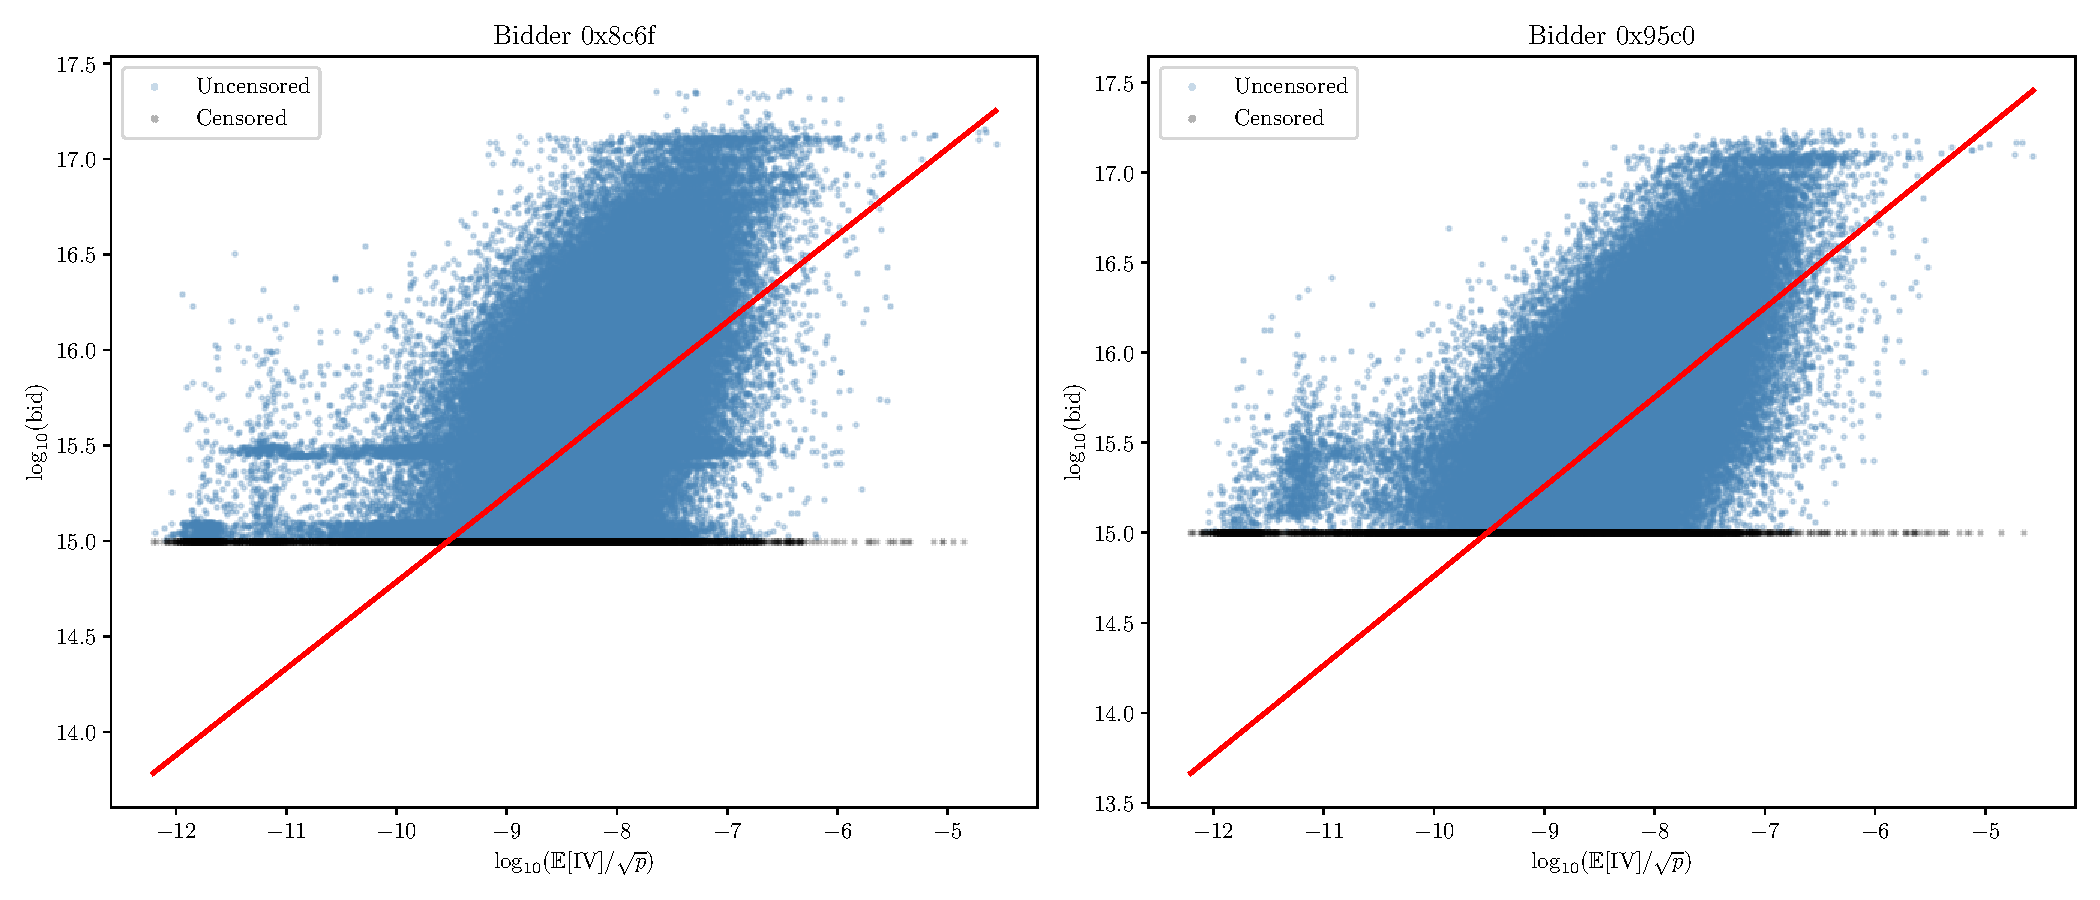
\includegraphics[width=0.9\linewidth]{images/plot_bid_vs_e_iv_sqrt_p.pdf}
    \caption{Scatter plot of each bidder's bids and price-adjusted integrated variance. Both are shown in log scale for visibility.}
    \label{fig:bid_vs_eiv}
\end{figure}

\Cref{tab:linear_nolag} shows the result of the estimates. For comparison, we also attach the result from the restricted model, which is identical to the original model except that the latent valuation depends only on $\widehat{\E[\IV]}$. This corresponds to the risk-neutral bidder's valuation. The first column corresponds to the restricted model, and the second to the previously introduced full model.

Across bidders, augmenting the specification with a variance term significantly improves the fit: LR tests are significant, and information criteria drop substantially. In the location equation, $\theta_1>0$ indicates that a higher expected IV is associated with higher bids, consistent with the view that the express-lane option is more valuable when arbitrage intensity rises. Conversely, $\theta_2<0$ on the standardized variance of the IV implies a risk discount: greater forecast uncertainty lowers valuations. Estimated tail parameters ($\nu\approx1.2$–$1.7$) confirm heavy-tailed residuals, justifying the Student-$t$ specification. \Cref{fig:bid_vs_eiv,fig:bid_vs_variv} provide comprehensive visualization of our result. 

Interestingly, the log-log variant of the reduced and full models yielded better results, although it lacks a theoretical justification. This may be due to the aforementioned scaling issues with the independent variables. The magnitude of the estimated mean and variance of IV spans across \(10^{-6}\) to \(10^{-3}\) and \(10^{-22}\) to \(10^{-12}\), respectively, and residuals on the samples with large estimated IV moments dominate in the process of MLE. See \cref{tab:log_nolag}.

\begin{figure}[htbp]
    \centering
    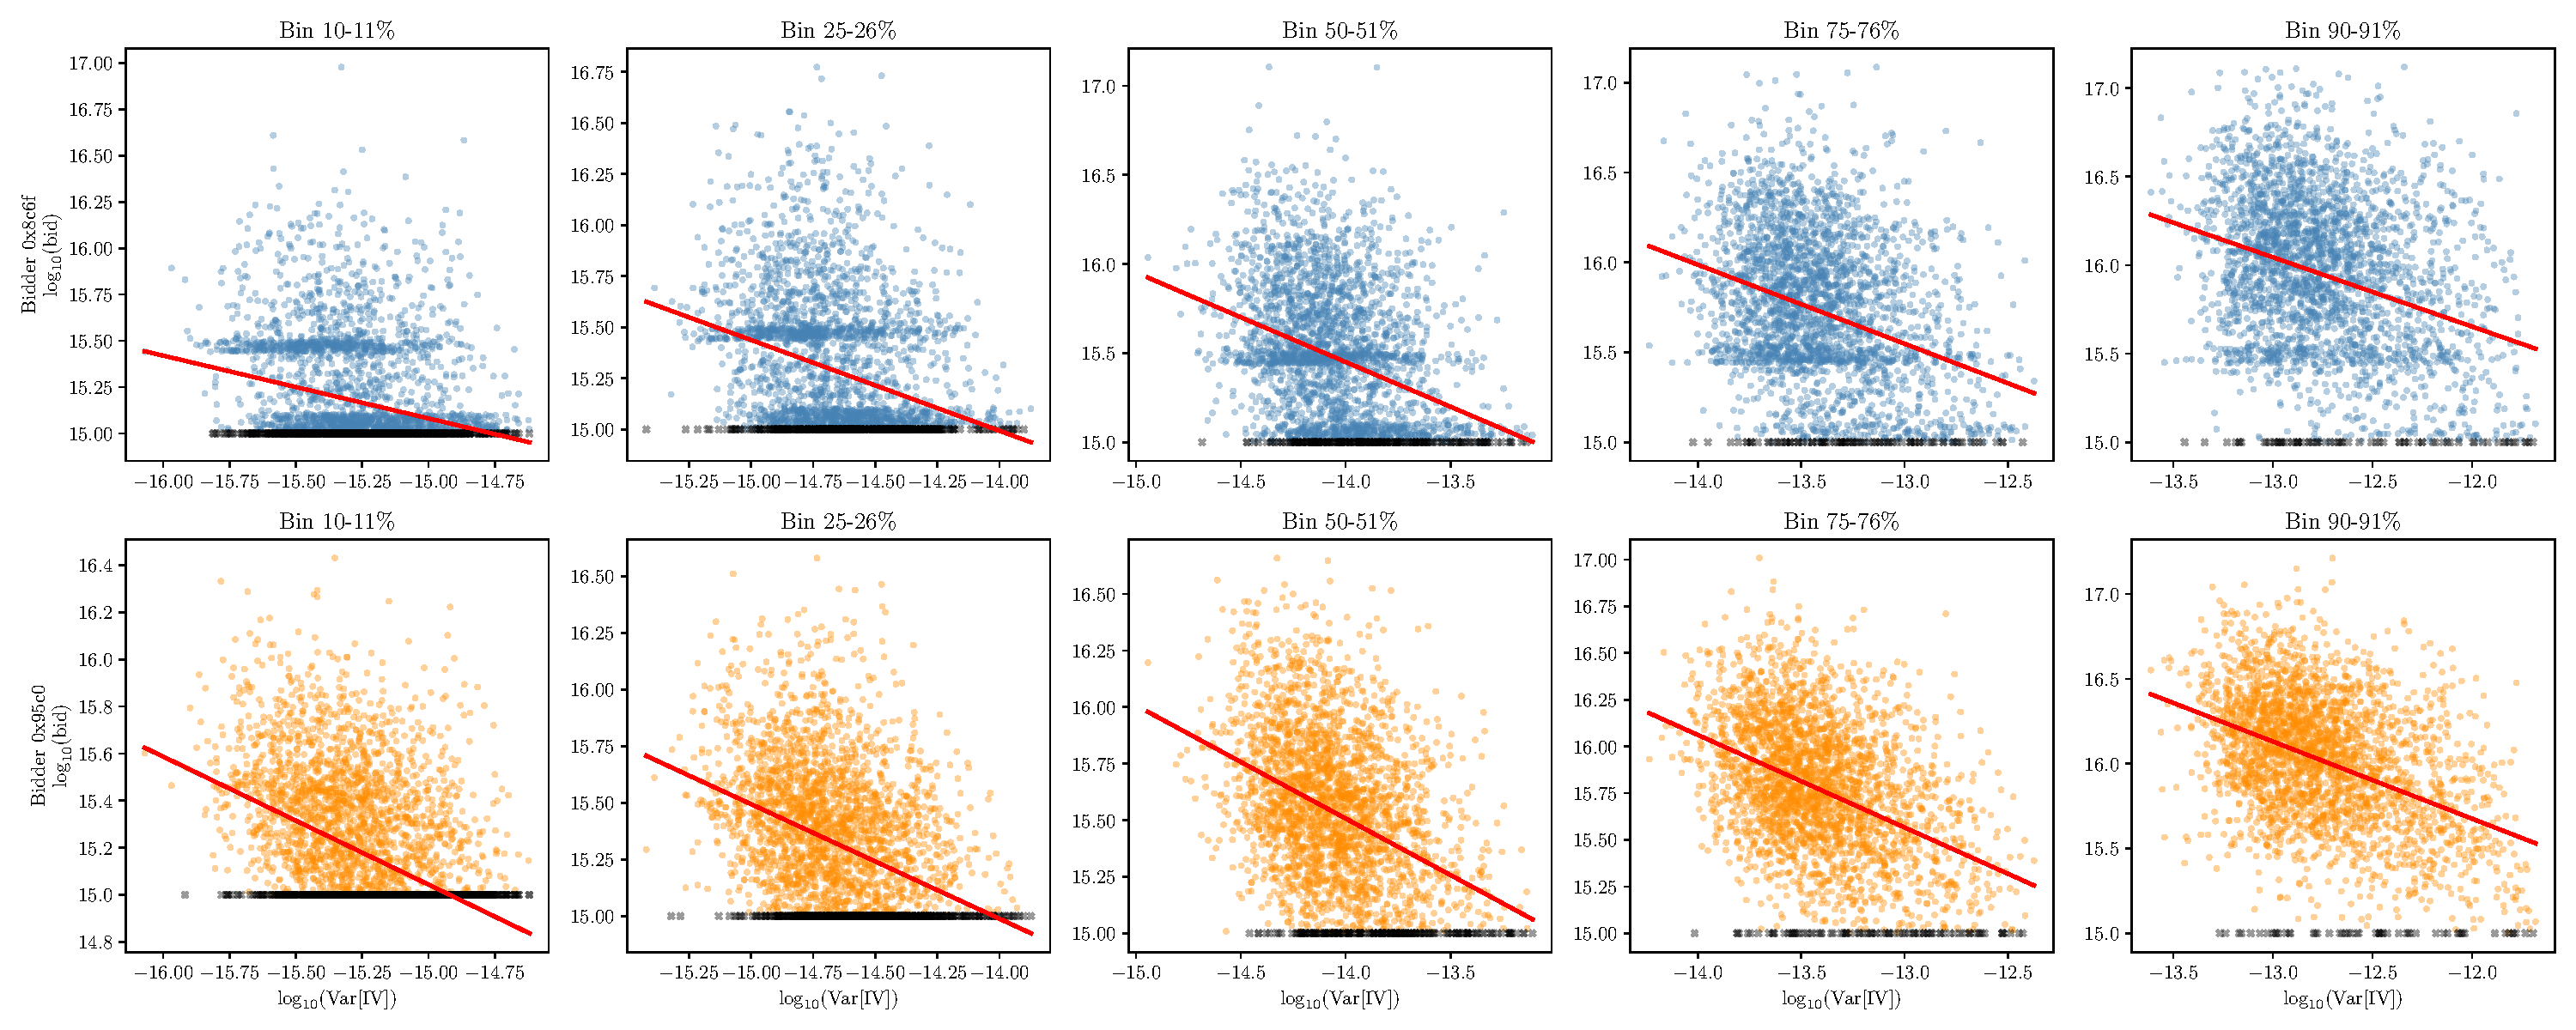
\includegraphics[width=0.9\linewidth]{images/plot_bid_vs_var_iv_conditional.pdf}
    \caption{Scatter plots of each bidder's bids grouped by percentile of $\E[\IV]/\sqrt P$. A heteroskedastic tobit regression was done for each subsample. For visibility, the figure is in log scale.}
    \label{fig:bid_vs_variv}
\end{figure}

\begin{table}[htbp]
\centering
\begin{tabular}{lcccc}
\toprule
 & \multicolumn{2}{c}{Bidder 0x8c6f} & \multicolumn{2}{c}{Bidder 0x95c0} \\
\cmidrule(lr){2-3} \cmidrule(lr){4-5}
Variable & Reduced & Full & Reduced & Full \\
\midrule
\multicolumn{5}{l}{\textit{Panel A: Location Coefficients}} \\
\addlinespace[0.5em]
Intercept ($\theta_0$) & 0.9878$^{***}$ & 0.9836$^{***}$ & 1.3691$^{***}$ & 1.1393$^{***}$ \\
 & (0.0011) & (0.0021) & (0.0061) & (0.0060) \\
E[IV]/$\sqrt{P}$ ($\theta_1$) & 0.3404$^{***}$ & 0.3472$^{***}$ & 0.3828$^{***}$ & 0.4421$^{***}$ \\
 & (0.0012) & (0.0014) & (0.0015) & (0.0017) \\
Var(IV) ($\theta_2$) & -- & -2.0792$^{***}$ & -- & -3.1878$^{***}$ \\
 & -- & (0.0340) & -- & (0.0460) \\
\addlinespace[0.5em]
\midrule
\multicolumn{5}{l}{\textit{Panel B: Scale Coefficients}} \\
\addlinespace[0.5em]
Intercept ($\gamma_0$) & -0.1690$^{***}$ & -2.2705$^{***}$ & 0.2718$^{***}$ & -1.4502$^{***}$ \\
 & (0.0052) & (0.0286) & (0.0041) & (0.0252) \\
$\log$(E[IV]/$\sqrt{P}$) ($\gamma_1$) & 0.5933$^{***}$ & 1.0895$^{***}$ & 0.4310$^{***}$ & 0.8572$^{***}$ \\
 & (0.0022) & (0.0072) & (0.0018) & (0.0064) \\
$\log$(Var(IV)) ($\gamma_2$) & -- & -0.3005$^{***}$ & -- & -0.2390$^{***}$ \\
 & -- & (0.0039) & -- & (0.0034) \\
\addlinespace[0.5em]
\midrule
\midrule
\multicolumn{5}{l}{\textit{Panel C: Model Fit Statistics}} \\
\addlinespace[0.5em]
Observations & 264959 & 264959 & 264959 & 264959 \\
Censored & 264959 & 264959 & 264959 & 264959 \\
Student $t$ $\nu$ & 1.23 & 1.30 & 1.55 & 1.70 \\
Log Likelihood & -729873.32 & -724012.17 & -724400.50 & -717011.02 \\
AIC & 1459756.64 & 1448038.34 & 1448810.99 & 1434036.03 \\
BIC & 1459809.08 & 1448111.75 & 1448863.43 & 1434109.44 \\
McFadden $R^2$ & 0.071 & 0.079 & 0.078 & 0.087 \\
\addlinespace[0.5em]
\midrule
\multicolumn{5}{l}{\textit{Panel D: Full vs Reduced Model Comparison}} \\
\addlinespace[0.5em]
$\Delta$ AIC (Full - Reduced) & \multicolumn{2}{c}{-11718.30} & \multicolumn{2}{c}{-14774.96} \\
$\Delta$ BIC (Full - Reduced) & \multicolumn{2}{c}{-11697.32} & \multicolumn{2}{c}{-14753.99} \\
LR Test $\chi^2$ (p-val) & \multicolumn{2}{c}{$11722.30^{***}$} & \multicolumn{2}{c}{$14778.96^{***}$} \\
\bottomrule
\end{tabular}
\caption{Heteroskedastic Tobit (Linear, t-dist Errors). $^{*}p<0.05$, $^{**}p<0.01$, $^{***}p<0.001$.}
\label{tab:linear_nolag}
\end{table}

\paragraph*{Robustness.}
We assess the robustness of the estimated relationships across different market conditions. To this end, we partition the dataset along both the temporal and regime dimensions. Specifically, the full sample is divided into (i) monthly subsamples from May through October and (ii) two volatility regimes (low and high, with median as threshold) delineated by the cross-sectional median of volatility. The regression model is then re-estimated separately for each subsample, and the corresponding estimates are reported in \cref{tab:tobit_subsample}.

Although the magnitude of the estimated coefficients varies across subsamples, the sign pattern is preserved: the coefficient on the variance of variance remains negative (interpreted as a discount) in all cases. A notable exception arises in the low-volatility regime, where the estimate of the coefficient on \(\theta_2\) is disproportionately large. While we do not have a definitive explanation for this outcome, we conjecture that it is attributable to a scaling issue. In particular, \(\widehat{\Var(\IV)}\) is approximately of the same order of magnitude as \(\widehat{\E[\IV]}^2\), with its minimum value on the order of \(10^{-22}\), and such extreme scaling potentially lead to estimation bias and numerical instability in some cases.

% TODO: restore the discussion of regression with lagged variables
To further verify our hypothesis without relying on the rational-expectations, i.e., the on-average correct forecasts assumption, we also ran a regression using lagged IV moment estimators, the estimated mean and variance of IV from the previous round, which are available to bidders at the time of bidding. For the result, see \cref{tab:linear_lagged,tab:log_lagged}. We found that not only does the discount remain persistent, but the overall goodness of fit also improves significantly for both linear and log-transformed models, suggesting the possibility of bidders relying on a simple AR(1) model instead of trying to precisely forecast the volatility distribution.

\subsection{Discussion}
The empirical findings reveal a statistically significant discount attributed to the inherent uncertainty (i.e., risk) associated with forecasting future volatility and the generated arbitrage revenue. 
% Especially, it is estimated that a \(1 \%\) increase in forecast variance leads to a \(0.4\%-0.5\%\) decrease in bids, which persists over various combinations of period, market regime, and bidder. 
This suggests that the efficiency of the ELA may diminish during periods of high market turbulence, not just because volatility is high, but because it becomes less predictable. This discount leads to lower bids relative to bidders' expected value of CEX-DEX arbitrage profit and, consequently, to a lower MEV capture rate. Further refinement of the ELA mechanism is required to mitigate this observed inefficiency. 
% Specifically, determining the optimal round length that minimizes the ratio of the variance of $\IV$ to its mean would be beneficial. That is, one should find the optimal round length $T^\ast$ which is defined as: \[
% T^\ast \equiv \min_{T} \frac{\Var\left(\int_0^T\sigma_s^2 ds\right)}{\E\left[\int_0^T\sigma_s^2 ds\right]}\quad.
% \] 

Given the challenges of accurately forecasting short-term volatility due to its low signal-to-noise ratio and non-stationarity, extending the round length to a longer duration, such as hourly or even daily, may be a more robust design. While longer horizons introduce other challenges, such as increased capital requirements, they may filter high-frequency noise and improve the signal-to-noise ratio of volatility forecasts. We also note that, instead of a seemingly arbitrary $0.001$ ETH, the reserve price should be set strategically to maximize expected revenue, balancing the guaranteed lower bound on payment with the probability of failing to attract any bidders.

Alternatively, a subscription-based model could be considered for simultaneously offering the express lane to multiple market participants. This approach has established precedents within traditional financial (TradFi) exchanges \cite{budish2024theory}, and recently launched perpetual exchanges such as Lighter and Paradex are adopting it as well\footnote{See \url{https://apidocs.lighter.xyz/docs/account-types} and \url{https://docs.paradex.trade/trading/trader-profiles\#fee-structure}.}.

\paragraph*{Limitations.}
Although the data support our hypotheses, our model has several limitations. Firstly, our model presents an oversimplified representation. Factors such as Total Value Locked (TVL) and liquidity near the current price significantly influence bidders' revenue; however, these elements are not incorporated into our model, which may introduce bias into our estimations. Secondly, data noise poses a challenge. Binance candles, generated from the last traded price, are susceptible to sudden price spikes from large market orders, thereby becoming decoupled from the true price. The use of future values as a proxy for the forecast also causes attenuation bias. We also remark that a significant portion of rounds being censored in samples and subsamples further weakens our claims, too.
